\documentclass{webofc}
\usepackage[varg]{txfonts}   % Web of Conferences font



\usepackage{todonotes}
\usepackage{tikz}
\usepackage{units}
\usepackage{pgfplots}
\usetikzlibrary{decorations.pathreplacing, patterns}
\pgfplotsset{compat=1.12}

\graphicspath{{./images/}}

% maybe use: https://github.com/olivierverdier/python-latex-highlighting/blob/master/pythonhighlight.sty

\begin{document}
%
\title{A Python upgrade to the GooFit package for parallel fitting}

\author{
	    \firstname{Henry}
        \lastname{Schreiner}\inst{1}\fnsep\thanks{\email{henry.fredrick.schreiner@cern.ch}}
        \and
        \firstname{Himadri}
        \lastname{Pandey}\inst{1}
        \and 
        \firstname{Michael D}
        \lastname{Sokoloff}\inst{1}
        \and
        \firstname{Bradley}
        \lastname{Hittle}\inst{2}
        \and 
        \firstname{Karen}
        \lastname{Tomko}\inst{2}
        \and 
        \firstname{Christoph}
        \lastname{Hasse}\inst{3}
}        % etc.

\institute{
	University of Cincinnati
\and
	Ohio Supercomputer Center
\and
	CERN / Technische Universit\"at Dortmund (DE)
}

\abstract{%
  The GooFit highly parallel fitting package for GPUs and CPUs has been substantially upgraded in the past year. Python bindings have been added to allow simple access to the fitting configuration, setup, and execution. A Python tool to write custom GooFit code given a (compact and elegant) MINT3/AmpGen amplitude description allows the corresponding C++ code to be written quickly and correctly. New PDFs have been added. The most recent release was built on top of the December 2017 2.0 release that added easier builds, new platforms, and a more robust and efficient underlying function evaluation engine.
}
%
\maketitle
%
\section{Introduction}
\label{intro}
High Energy Physics experiments around the world are producing record amounts of data. Existing tools, such as the RooFit fitting framework, provide flexible and powerful abstractions for building distributions to fit that data with, but this power comes at a cost; this is computationally expensive, and often only runs on a single core. Modern architectures provide many cores, as well as new computing paradigms, such as GPUs, that provide significant new potential for high performance computations, but are non-trivial for the physicst to use to build distributions in the description style familiar to him.

GooFit is a high-performance multi-thread and GPU ready framework providing a similar syntax to RooFit developed at the University of Cincinnati in 2013~\cite{lib:GooFit:main}. It provided composition of model pieces in the same manor as RooFit, but was powered by GPUs. It also provided ready to use models for common Probability Distribution Functions (PDFs), as well as specialized three body physics models. The GooFit 2.0 release~\cite{lib:GooFit} added a simpler build process, making it easy for users to pick up and run GooFit code, and combined work from several forks, providing more physics models and more features.

The next two releases of GooFit, bringing us up to version 2.2, will be the topic of our discussion. The most notable new change is the addition of fully functioning Python bindings, allowing users to code the composition of PDFs in a dynamic scripting language, opening up new possibilities for quick modeling and interesting interactions with other Python libraries, such as for plotting. Other changes include a new indexing system, which makes PDFs easier to write, and provides some small performance benefits on GPUs. A prototype for a uniform decay language, shared with other packages such as AmpGen~\todo{REF}, provides a powerful new frontend that can be used for user code.

\section{GooFit Performance}

\begin{figure*}
	\centering
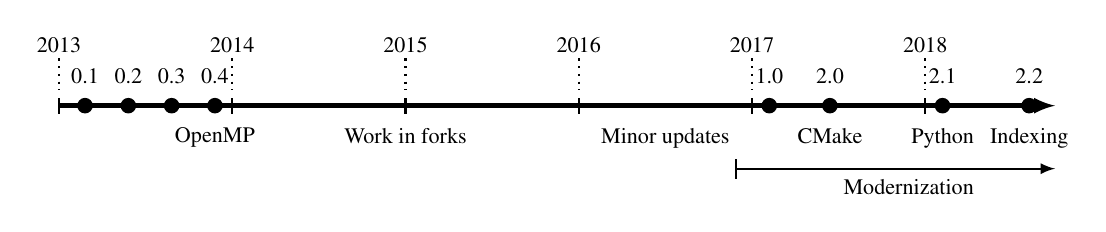
\begin{tikzpicture}[xscale=1.1,
goonode/.style={fill=black, circle, minimum size=1.25ex, inner sep=0},
version/.style={above=1ex, black},
events/.style={below=1ex, black},
every node/.style={font=\footnotesize}
]
\draw [-latex, ultra thick, black] (0,0) -- (11.5,0);
\draw [|-latex, thick, black] (7.8,-.8) -- (11.5,-.8) node [midway, below, xshift=.5em] {Modernization};

\foreach \x in {2013,...,2018} {
	\node at (2*\x-2*2013,0) [above=3.5ex, black] {\x};
	\draw [thick, black] (2*\x-2*2013,-.1) -- (2*\x-2*2013,.1);
	\draw [thick, dotted, black] (2*\x-2*2013,.6) -- (2*\x-2*2013,.2);
}

\node (v01) at (.3,0) [goonode] {};
\node at (v01) [version] {0.1};

\node (v02) at (.8,0) [goonode] {};
\node at (v02) [version] {0.2};

\node (v03) at (1.3,0) [goonode] {};
\node at (v03) [version] {0.3};

\node (v04) at (1.8,0) [goonode] {};
\node at (v04) [events] {OpenMP};
\node at (v04) [version] {0.4};

\node at (4,0) [events] {Work in forks};

\node (v10) at (8.2,0) [goonode] {};
\node at (7,0) [events] {Minor updates};
\node at (v10) [version] {1.0};

\node (v20) at (8.9,0)  [goonode] {};
\node at (v20) [events] {CMake};
\node at (v20) [version] {2.0};

\node (v21) at (10.2,0)  [goonode] {};
\node at (v21) [events] {Python};
\node at (v21) [version] {2.1};

\node (v22) at (11.2,0)  [goonode] {};
\node at (v22) [events] {Indexing};
\node at (v22) [version] {2.2};
\end{tikzpicture}%
\caption{Timeline of GooFit development. Key points are version 2.0: New build system, C++11, and 4-body time dependent analyses support; version 2.1: Python bindings using Pybind11; and version 2.2: new indexing (and lots of Python improvements).}
\label{fig-history}
\end{figure*}

\begin{figure}[h]
	\centering
	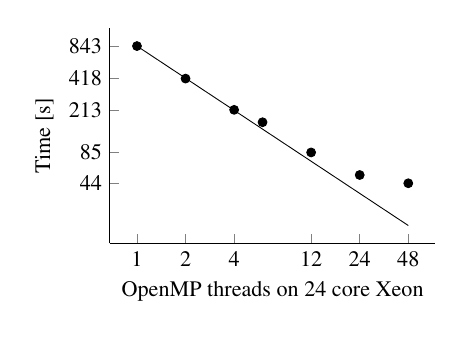
\begin{tikzpicture}[scale=.8]
	\begin{loglogaxis}[
	axis x line*=bottom,
	axis y line*=left,
	xlabel={OpenMP threads on 24 core Xeon},
	ylabel={Time [s]},
	width=6.75cm,
	height=5cm,
	log ticks with fixed point,
	xtick={1,2,4,12,24,48},
	ytick={44,85,213,418,843}
	]
	\addplot[domain=1:48] {843/x};
	\addplot [color=black, only marks] coordinates {%
		(1,843)
		(2,418)
		(4, 213)
		(6,163)
		(12, 84.98)
		(24, 52.22)
		(48,43.7)
	};
	
	\end{loglogaxis}
	\end{tikzpicture}
	\caption{$\pi\pi\pi^0$, 16 time-dependent amplitudes. Original RooFit code: \unit[19,489]{s} single core. 40 free par.\ and 100,000+ events.}
	\label{fig-pipipi0}
\end{figure}

\begin{figure}[h]
	\centering
	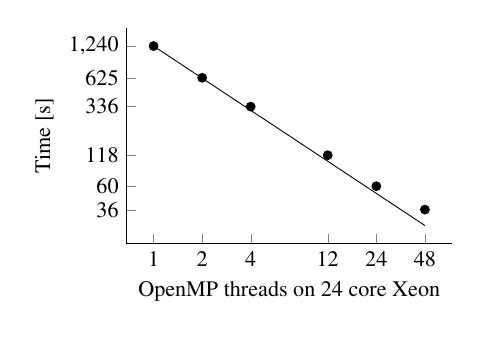
\begin{tikzpicture}[scale=.8]
	\begin{loglogaxis}[
	axis x line*=bottom,
	axis y line*=left,
	xlabel={OpenMP threads on 24 core Xeon},
	ylabel={Time [s]},
	width=6.75cm,
	height=5cm,
	log ticks with fixed point,
	xtick={1,2,4,12,24,48},
	ytick={36, 60, 118, 336, 625, 1240}
	]
	\addplot[domain=1:48] {1239.565/x};
	\addplot [color=black, only marks] coordinates {%
		(1,1239.5650)
		(2,625.0800)
		(4,335.6160)
		(12,117.7198)
		(24,60.3316)
		(48,36.4039)
	};
	
	\end{loglogaxis}
	\end{tikzpicture}
	\caption{ZachFit: $M (D^{*+})-M (D^0)$. 142,576 events in unbinned fit.}
	\label{fig-zachfit}
\end{figure}

\begin{table}
	\centering
	\begin{tabular}{c|c|c|c}
		Number of Cores & Hardware & Pipipi0 & ZachFit \\
		\hline
2 Cores &           Core 2 Duo & \unit[1,159]{s} & \unit[738]{s} \\
GPU &  GeForce GTX 1050 Ti & \unit[86.4]{s}& \unit[60.3]{s}   \\
GPU &            Tesla K40 & \unit[64.0]{s} & \unit[60.3]{s} \\
MPI \& GPU & Tesla K40 $\times 2$ & \unit[39.3]{s} & \unit[54.3]{s} \\
GPU &           Tesla P100 & \unit[20.3]{s}& \unit[23.5]{s} \\
	\end{tabular}
\caption{GPU performance comparison.}
\label{tab-zachfit}
\end{table}


\section{Python Bindings}
\label{sec-py}

The 

\section{The New Indexing System}
\label{sec-ind}

\begin{figure}
	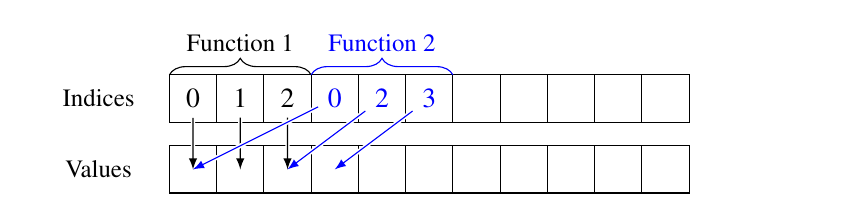
\begin{tikzpicture}[scale=.6,
	arr/.style={-latex, preaction={draw, -latex, white, ultra thick}}]
	\path[use as bounding box] (-3,-1.5) rectangle (14, 2);
	
	\foreach \x in {0,...,10} {
		\draw (\x,0) rectangle (\x+1,1);
		\draw (\x,-1.5) rectangle (\x+1,-.5);
	}
	\node at (-1.5,.5) {\small Indices};
	\node at (-1.5,-1) {\small Values};
	
	\node (a) at (0.5,.5) {0};
	\coordinate (A) at (0.5, -1);
	\draw [arr] (a) -- (A);
	
	\node (b) at (1.5,.5) {1};
	\coordinate (B) at (1.5, -1);
	\draw [arr] (b) -- (B);
	
	\node (c) at (2.5,.5) {2};
	\coordinate (C) at (2.5, -1);
	\draw [arr] (c) -- (C);
	
	\draw [decorate, decoration={brace,amplitude=6pt},xshift=0pt,yshift=0pt]
	(0,1) -- (3,1) node [black,midway,yshift=.4cm] {\small Function 1};
	
	
	\node [blue] (d) at (3.5,.5) {0};
	\draw [blue, arr] (d) -- (A);
	
	\node [blue] (e) at (4.5,.5) {2};
	\draw [blue, arr] (e) -- (C);
	
	\node [blue] (f) at (5.5,.5) {3};
	\coordinate (D) at (3.5, -1);
	\draw [blue, arr] (f) -- (D);
	
	\draw [blue, decorate, decoration={brace,amplitude=6pt},xshift=0pt,yshift=0pt]
	(3,1) -- (6,1) node [blue,midway,yshift=.4cm] {\small Function 2};
	
	\end{tikzpicture}
	\caption{An example of the classic GooFit indexing system.}
	\label{fig-indexing-classic}
\end{figure}

\begin{figure}
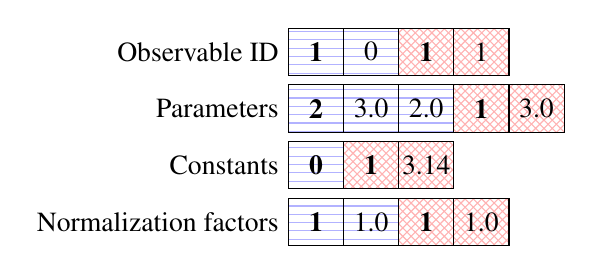
\begin{tikzpicture}[xscale=.7, yscale=.6,
first/.style={pattern=horizontal lines, pattern color=blue!30!white},
second/.style={pattern=crosshatch, pattern color=red!30!white},
ind/.style={font=\bf}]
\begin{scope}
\node at (0,0.5) [left] {Observable ID};
\draw [first, ind] (0,0) rectangle (1,1) node [midway] {1};
\draw [first] (1,0) rectangle (2,1) node [midway] {0};
\draw [second, ind] (2,0) rectangle (3,1) node [midway] {1};
\draw [second] (3,0) rectangle (4,1) node [midway] {1};
\end{scope}
\begin{scope}[yshift=-1.2cm]
\node at (0,0.5) [left] {Parameters};
\draw [first, ind] (0,0) rectangle (1,1) node [midway] {2};
\draw [first] (1,0) rectangle (2,1) node [midway] {3.0};
\draw [first] (2,0) rectangle (3,1) node [midway] {2.0};
\draw [second, ind] (3,0) rectangle (4,1) node [midway] {1};
\draw [second] (4,0) rectangle (5,1) node [midway] {3.0};
\end{scope}
\begin{scope}[yshift=-2.4cm]
\node at (0,0.5) [left] {Constants};
\draw [first, ind] (0,0) rectangle (1,1) node [midway] {0};
\draw [second, ind] (1,0) rectangle (2,1) node [midway] {1};
\draw [second] (2,0) rectangle (3,1) node [midway] {3.14};
\end{scope}
\begin{scope}[yshift=-3.6cm]
\node at (0,0.5) [left] {Normalization factors};
\draw [first, ind] (0,0) rectangle (1,1) node [midway] {1};
\draw [first] (1,0) rectangle (2,1) node [midway] {1.0};
\draw [second, ind] (2,0) rectangle (3,1) node [midway] {1};
\draw [second] (3,0) rectangle (4,1) node [midway] {1.0};
\end{scope}
\end{tikzpicture}
\caption{An example of the new GooFit indexing system.}
\label{fig-indexing-new}
\end{figure}

The indexing system has been updated to provide improved GPU performance. The indexing system in GooFit needs to track the Variables, Observables, and any constants used by any combination of PDFs. This information is packed into four separate buffers. The primary index buffer provides either a constant integer value, or contains the index into one of the three subsequent buffers which contained events, parameters, or floating-precision constants~\cite{lib:GooFit:main}. For simple PDFs, performance is not an issue due to the amount of memory. The indexing memory stays small, and can be cached quickly. As more PDFs are involved in the fit, complexity is added causing the indexing memory to get quite large with requests becoming random. For GPUs this is a problematic issue which causes a large overhead reading similar blocks of memory from global memory due to the size of the L1 cache. Using the new indexing system improves this access pattern by having memory reads behave coherently. A side effect of the new indexing system is duplicated memory for a specific Variable or Observable. The performance improvement at the cost of this duplicating memory has a larger impact on performance by providing a linear memory access for each PDF.

The second improvement with the indexing system provides is developing and testing PDFs as well by providing a method for testing that indices specific in PDF construction match with the device function. Helper functions have been added allowing for registered Variables and Observables to also return the index that needs to be used within the device function. This provides a simpler mechanism for creating and debugging new PDFs by verifying indices in the device function. 

An additional change provided with the indexing update is the ParameterContainer structure which provides a consistent method for accessing all indexed values. Each device function requires a ParameterContainer reference, and each device function will need to increment the internal structure. Any additional caching techniques are hidden in this structure.

\begin{table}
	\centering
	\begin{tabular}{ |r|r|r| }
		\hline
			 & GooFit 2.0 (s) & GooFit 2.2 (s) \\
		\hline
			Dalitz [100,000 events] & 3.12221 & 1.70781 \\
		\hline
			Daltiz [10,000,000 events] & 317.347 & 130.282 \\
		\hline
	\end{tabular}
	\caption{Performance comparisons of GooFit 2.0 versus GooFit 2.2 including the new indexing system.}
	\label{table:1}
\end{table}

\begin{figure}
	 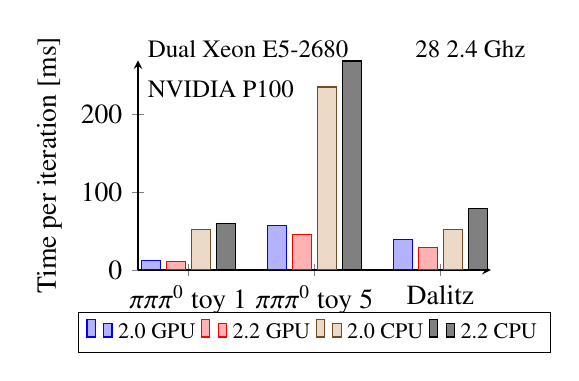
\begin{tikzpicture}
	\begin{axis}[
	ylabel={Time per iteration [ms]},
	xtick={1,2,3},
	xticklabels={$\pi\pi\pi^0$ toy 1,$\pi\pi\pi^0$ toy 5,Dalitz},
	legend style={at={(0.5,-0.2),font=\footnotesize},
		anchor=north,legend columns=-1},
	width=.5\textwidth,
	height=.35\textwidth,
	ybar,
	bar width=7pt,
	axis x line=bottom,
	axis y line=left,
	ymin=0,
	ymax=270,
	xmin=.6,
	xmax=3.4
	]
	% 2.0 GPU
	\addplot coordinates {
		(1,12.322)
		(2,57.259)
		(3,38.811)
	};
	% 2.2 GPU
	\addplot coordinates {
		(1,10.412)
		(2,45.358)
		(3,29.275)
	};
	\addplot coordinates {
		(1,51.99)
		(2,235.69)
		(3,52.223)
	};
	\addplot coordinates {
		(1,59.615)
		(2,269.16)
		(3,79.276)
	};
	\legend{2.0 GPU,2.2 GPU,2.0 CPU,2.2 CPU}
	\end{axis}
	\node at(0,2.8) [right] {\small Dual Xeon E5-2680};
	\node at(3.4,2.8) [right] {\small 28 2.4~Ghz};
	\node at(0,2.3) [right] {\small NVIDIA P100};
	\end{tikzpicture}
	\label{figure-newindexspeed}
	\caption{New indexing system.}
\end{figure}

Table \ref{table:1} provides a performance comparison between the old indexing system in GooFit 2.0 and the new indexing system found in GooFit 2.2. The results show that providing more coherent memory reads improves the performance by a factor of 2.4 in the large event case, with a 82\% improvement with a small dataset.

\section{A Uniform Decay Language}
\label{sec-ampgen}
More here.

\begin{figure}
	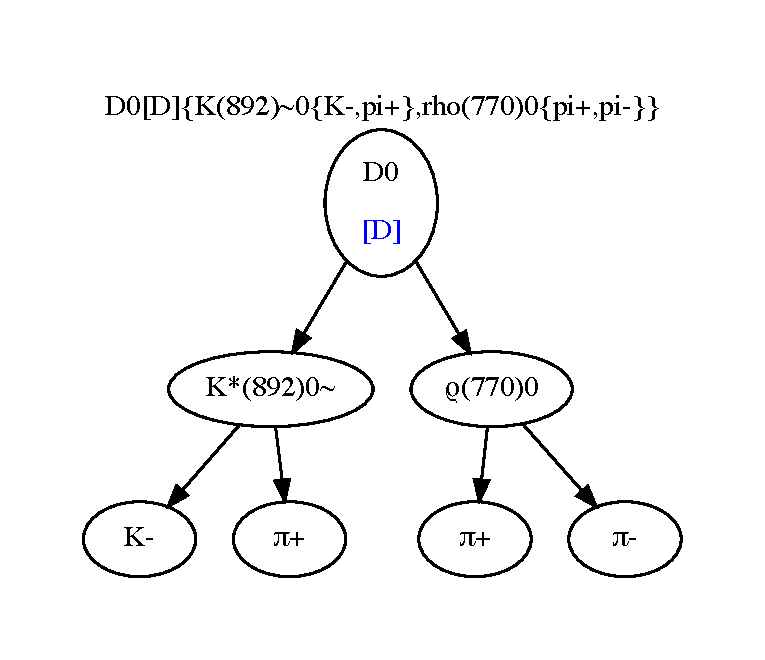
\includegraphics[width=.5\textwidth]{LineExample}
	\label{figure-ampgen}
	\caption{Example of decay from DecayLanugage.}
\end{figure}

\section{Summary}
\label{sec-summary}
More here.

%For one-column wide figures use syntax of figure~\ref{fig-1}
%\begin{figure}[h]
% Use the relevant command for your figure-insertion program
% to insert the figure file.
%\centering
%\includegraphics[width=1cm,clip]{tiger}
%\caption{Please write your figure caption here}
%\label{fig-1}       % Give a unique label
%\end{figure}

%For two-column wide figures use syntax of figure~\ref{fig-2}
%\begin{figure*}
%\centering
%% Use the relevant command for your figure-insertion program
%% to insert the figure file. See example above.
%% If not, use
%\vspace*{5cm}       % Give the correct figure height in cm
%\caption{Please write your figure caption here}
%\label{fig-2}       % Give a unique label
%\end{figure*}
%
%For figure with sidecaption legend use syntax of figure
%\begin{figure}
%% Use the relevant command for your figure-insertion program
%% to insert the figure file.
%\centering
%\sidecaption
%\includegraphics[width=5cm,clip]{tiger}
%\caption{Please write your figure caption here}
%\label{fig-3}       % Give a unique label
%\end{figure}

%For tables use syntax in table~\ref{tab-1}.
%\begin{table}
%\centering
%\caption{Please write your table caption here}
%\label{tab-1}       % Give a unique label
%% For LaTeX tables you can use
%\begin{tabular}{lll}
%\hline
%first & second & third  \\\hline
%number & number & number \\
%number & number & number \\\hline
%\end{tabular}
%% Or use
%\vspace*{5cm}  % with the correct table height
%\end{table}
%
% BibTeX or Biber users please use (the style is already called in the class, ensure that the "woc.bst" style is in your local directory)
\bibliography{goofit}
%
% Non-BibTeX users please use
%
%\begin{thebibliography}{}
%%
%% and use \bibitem to create references.
%%
%
%\bibitem{GooFit}
%R Andreassen et al.
%\textit{GooFit: A library for massively parallelising maximum-likelihood fits}
%Phys.: Conf. Ser. 513 052003 (2014)
%
%\bibitem{RefJ}
%% Format for Journal Reference
%Journal Author, Journal \textbf{Volume}, page numbers (year)
%% Format for books
%\bibitem{RefB}
%Book Author, \textit{Book title} (Publisher, place, year) page numbers
%% etc
%\end{thebibliography}

\end{document}

% end of file template.tex

<div id='footer'><table width='100%'><tr><td class='right'><a href='http://fusioninventory.org/'><span class='copyright'>FusionInventory 9.1+1.0 | copyleft <img src='/glpi/plugins/fusioninventory/pics/copyleft.png'/>  2010-2016 by FusionInventory Team</span></a></td></tr></table></div>
